%%% Research Diary - Entry
\documentclass[11pt,a4paper]{article}

% Working date: The date this entry is describing. Not necessary the date of last edit.
\newcommand{\workingDate}{\textsc{2019 $|$ May $|$ 06}}

% Name and institution must preceed call to researchdiary.sty package
\newcommand{\userName}{Pierre Bréchet}
\newcommand{\institution}{TUM}

% The guts and glory
\usepackage{research_diary}
\usepackage{usrcmd}
\bibliography{bibliography}

% Begin document.
% Use \logoPNG or \logoEPS. If compiling with PDFTeX, use \logoPNG
\begin{document}
% \logoPNG

{\Huge May  6}

\section*{Training gaussians}

Back to training on gaussians with informative and anti-informative models.

Batch normalization improves the learning in this case as well. As recommended by DCGAN, avoid using batch normalization for the first layer of discriminators.

\paragraph{Update} Is using batchnormalization in G as well useful ? ALI does not use batchnorm in the discriminator, but in the generator only...

\subsection*{Anti-informative reformulation}

Using the symmetrical formulation of the anti-informative regularization, the results are not outstanding...

\paragraph{Bug corrected} Evaluation of the generator must be enclosed withing \texttt{G.eval() ... G.train()} if batch normalization is used in the generator.

\paragraph{Dev} Changed the behavious of Gaussian data generation, used to whiten the data
by dividing by the standard deviation, not anymore. Set the grid following
\cite{Dumoulin2016}.

\paragraph{Tests} Testing the primal anti-informative regularization, the informative regularization (all with Sinkhorn), the InfoGAN model.

\section*{Cropping the CelebA}

\paragraph{Cropped dataset}

The repo of infogan does not provide the CelebA dataset used in the paper
experiments. \\

Moreover, none (?) of the listed repositories for InfoGAN
\footnote{\url{https://paperswithcode.com/paper/infogan-interpretable-representation-learning}}
contains the code for the cropped CelebA dataset. Therefore, the images are
cropped following

Update: check ALI \footnote{\url{https://ishmaelbelghazi.github.io/ALI/}} for the CelebA and other dataset (code is available, rely on some libraries) \\

The images are therefore manually cropped to cover a  pixel region
of width 40 pixels and respected ratio 218/178 (original images are 178x218).
Original images are centered around the eyes, cropped images are more centered
around the nose. \\

Images are then rezised to 64x64, and saved in a HDF5 file.
% \begin{figure}[!htbp]
   \centering
\begin{subfigure}[t]{0.48\textwidth}
   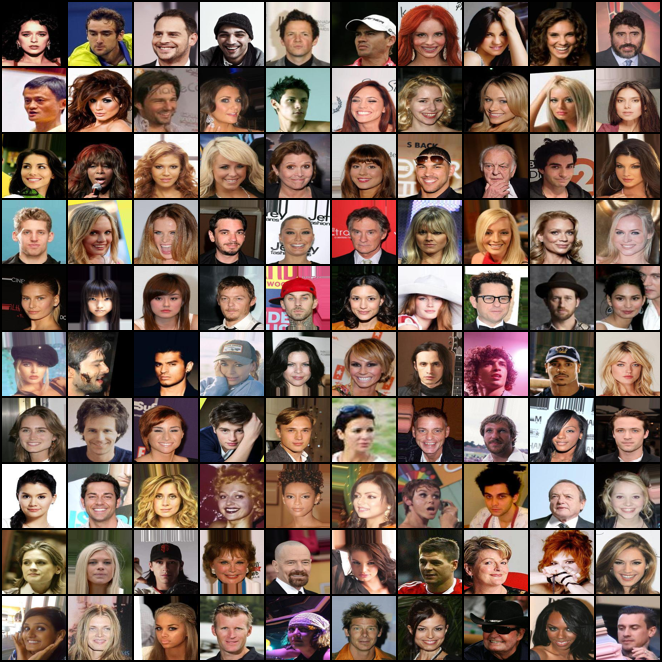
\includegraphics[width=\textwidth,center]{2019-05-06/celeba-crop/a_original.png}
   \caption{a_original.}
   \label{fig:2019-05-06_celeba-crop-a}
\end{subfigure}
\begin{subfigure}[t]{0.48\textwidth}
   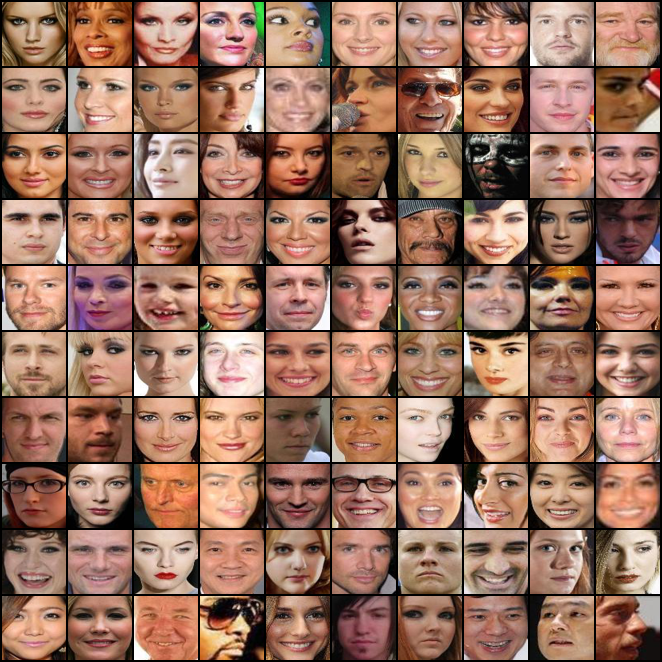
\includegraphics[width=\textwidth,center]{2019-05-06/celeba-crop/b_cropped.png}
   \caption{b_cropped.}
   \label{fig:2019-05-06_celeba-crop-b}
\end{subfigure}
   \caption{Original (left) vs cropped (right) CelebA}
   \label{fig:2019-05-06_celeba-crop}
\end{figure}

\paragraph{Bug?} There might be a bug in reading (cropped and regular) CelebA from the HDF5 file when using multiple threads. Or it is just displaying images from the file that is not always working.

\begin{figure}[!htbp]
   \centering
\begin{subfigure}[t]{0.48\textwidth}
   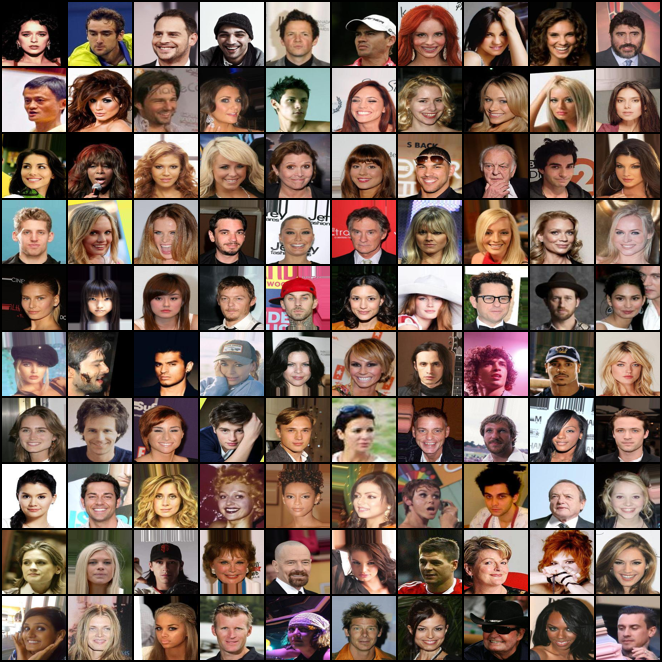
\includegraphics[width=\textwidth,center]{2019-05-06/celeba-bug/a_normal.png}
   \caption{a_normal.}
   \label{fig:2019-05-06_celeba-bug-a}
\end{subfigure}
\begin{subfigure}[t]{0.48\textwidth}
   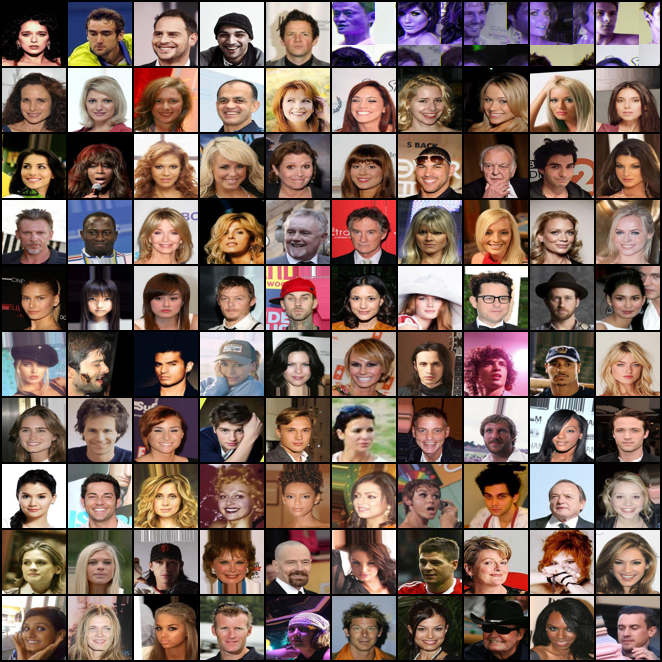
\includegraphics[width=\textwidth,center]{2019-05-06/celeba-bug/b_bug.png}
   \caption{b_bug.}
   \label{fig:2019-05-06_celeba-bug-b}
\end{subfigure}
\begin{subfigure}[t]{0.48\textwidth}
   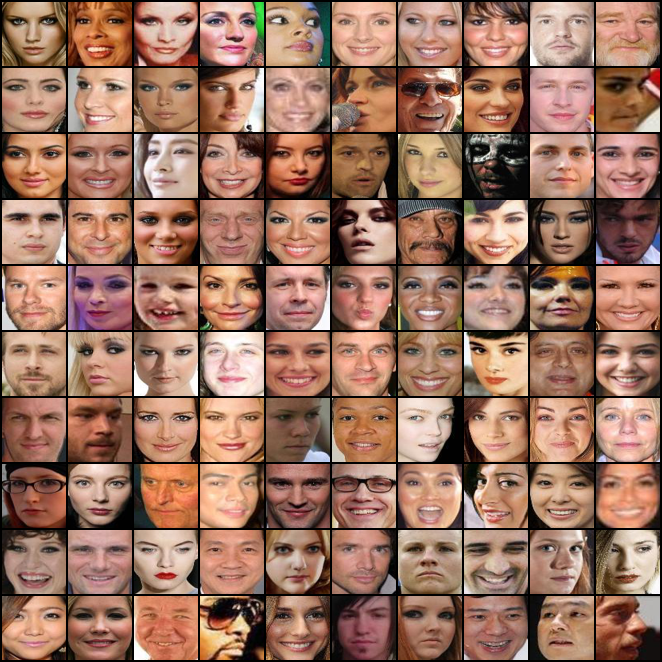
\includegraphics[width=\textwidth,center]{2019-05-06/celeba-bug/c_crop_normal.png}
   \caption{c_crop_normal.}
   \label{fig:2019-05-06_celeba-bug-c}
\end{subfigure}
\begin{subfigure}[t]{0.48\textwidth}
   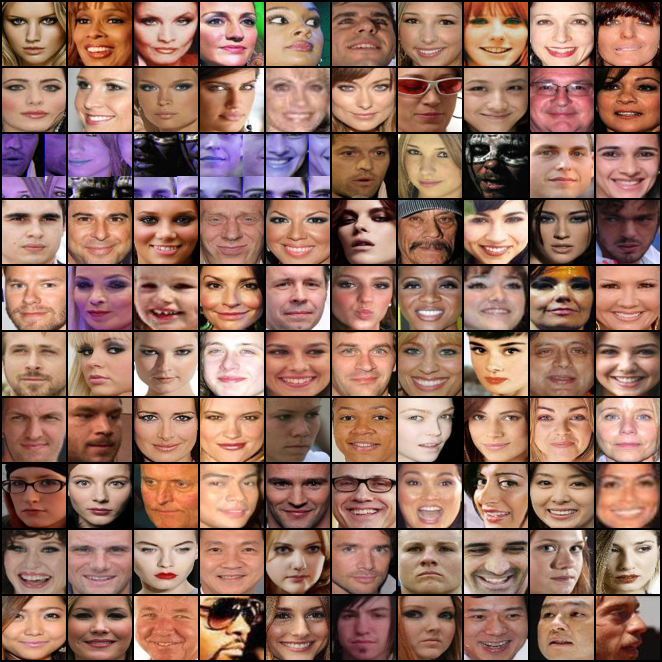
\includegraphics[width=\textwidth,center]{2019-05-06/celeba-bug/d_crop_bug.png}
   \caption{d_crop_bug.}
   \label{fig:2019-05-06_celeba-bug-d}
\end{subfigure}
   \caption{Normal (left) vs bugged (right) visualization of the cropped CelebA dataset. The bug disappears when not using mutli-thread processing.}
   \label{fig:2019-05-06_celeba-bug}
\end{figure}

\printbibliography{}
\end{document}
